\model{Common Methods}

Classes are often used to represent abstract data types, such as \java{Color} or \java{Point}:

\begin{center}
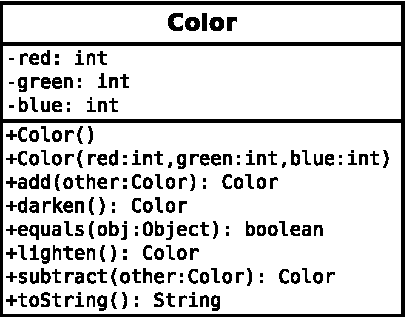
\includegraphics{Color.pdf}  % immutable
~~~~~
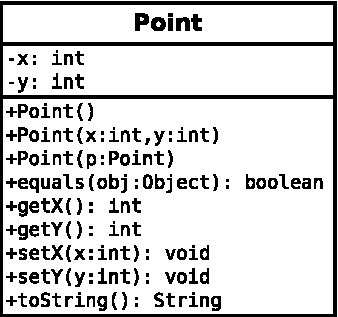
\includegraphics{Point.pdf}  % mutable
\end{center}

As shown in the UML diagrams, classes generally include the following kinds of methods (in addition to others):

\begin{itemize}[itemsep=0pt]
\item \textbf{constructor} methods that initialize new objects
\item \textbf{accessor} methods (getters) that return attributes
\item \textbf{mutator} methods (setters) that modify attributes
%\item \textbf{object} methods such as \java{equals} and \java{toString}
%\item \textbf{utility} methods which are generally static
\end{itemize}

%Note: The \java{Color} class does not have getters and setters.


\quest{15 min}


\Q Identify the constructors for the \java{Color} class.
What is the difference between them?
%What arguments do they take?

\begin{answer}[3em]
There are two constructors: one that takes no parameters (the default constructor), and one that takes three integers for the RGB values.
\end{answer}


\Q What kind of constructor does the \java{Point} class have that the \java{Color} class does not?
%Explain the purpose of such a constructor.

\begin{answer}[3em]
The \java{Point} class also has a copy constructor: one that ``copies'' the values of another object.
\end{answer}


\Q Identify an accessor method in the \java{Point} class.

\begin{enumerate}
\item What is the name of the method? \ans{{\tt getX} or {\tt getY}}
\item Which instance variable does it get? \ans{{\tt this.x} or {\tt this.y}}
\item What arguments does the method take? \ans{none}
\item What does the method return? \ans{The value of \java{x} or \java{y}}
\end{enumerate}


\Q Identify a mutator method in the \java{Point} class.

\begin{enumerate}
\item What is the name of the method? \ans{{\tt setX} or {\tt setY}}
\item Which instance variable does it set? \ans{{\tt this.x} or {\tt this.y}}
\item What arguments does the method take? \ans{The value of \java{x} or \java{y}}
\item What does the method return? \ans{nothing}
\end{enumerate}


\Q How would you define accessor methods for each attribute of the \java{Color} class?
Write your answer using UML syntax.

\begin{answer}[5em]
\begin{javaans}
+getRed(): int
+getGreen(): int
+getBlue(): int
\end{javaans}
\end{answer}


\Q How would you define mutator methods for each attribute of the \java{Color} class?
Write your answer using UML syntax.

\begin{answer}[5em]
\begin{javaans}
+setRed(red:int)
+setGreen(green:int)
+setBlue(blue:int)
\end{javaans}
\end{answer}


\Q \label{immutable}
The \java{Color} class does not provide any accessors or mutators.
Instead, it provides methods that return new \texttt{Color} objects.
Why do you think the class was designed this way?

\begin{answer} [5em]
Other than the constructor, there are no methods that change the \texttt{red}, \texttt{green}, and \texttt{blue} values.
This design makes the class immutable, which means that objects can be reused.
The \java{String} class is also designed this way.
\end{answer}
